\documentclass{standalone}
\usepackage{tikz}
\usepackage{amssymb}
\usetikzlibrary{automata, positioning}

\begin{document}
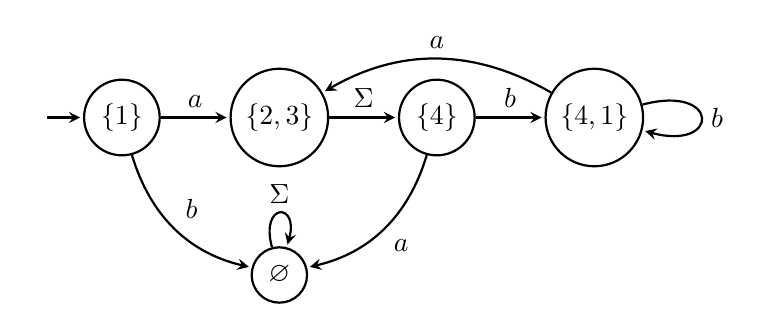
\begin{tikzpicture}[%
    >=stealth,
    shorten >=1pt,
    node distance=2cm,
    on grid,
    auto,
    state/.append style={minimum size=2em},
    thick
  ]

  \node[state, initial, initial text = {}] (A) {$\{1\}$};
  \node[state] (B) [right of=A] {$\{2, 3\}$};
  \node[state] (C) [right of=B] {$\{4\}$};
  \node[state] (D) [right of=C] {$\{4, 1\}$};
  \node[state] (E) [below of=B] {$\varnothing$};

  \path[->]
              (A)         edge [          ] node {$a$} (B)
              (A)         edge [bend right] node {$b$} (E)
              (B)         edge [         ]  node {$\Sigma$} (C)
              (C)         edge [bend left]  node {$a$} (E)
              (C)         edge [          ] node {$b$} (D)
              (D)         edge [bend right] node[above] {$a$} (B)
              (D)         edge [loop right] node {$b$} (D)
              (E)         edge [loop above] node {$\Sigma$} (E);
\end{tikzpicture}
\end{document}